% Conversion-channel stability probe and chain-time perturbativity gate.
% Source: design notes from the #323 Stage C investigation.
% Uses macros from preamble.tex

\section{Stability Probe and Inline Perturbativity Gate}
\label{sec:stability-probe}

The conversion-channel stability probe is the first stage in a
three-step rejection cascade
(\Cref{tab:stability-cascade}) that filters out parameter samples
whose linearised simulation cannot legitimately represent the
underlying physics. It runs at chain time, before any simulation, and
combines with an inline perturbativity gate after the simulation to
produce contamination-free Bayesian chains: every accepted sample has
been confirmed to (a) admit a numerically stable linearised evolution
and (b) yield a conversion probability inside the Hwang--Noh
perturbative window.

\begin{table}[ht]
\centering
\begin{tabular}{lll}
\toprule
\textbf{Stage} & \textbf{Cost} & \textbf{Rejects} \\
\midrule
Probe pre-flight (all $k$ Pad\'e) & $\sim$ ms / sample & tachyonic linearisation \\
PDE simulation & $\sim$ s / sample & numerical divergence (\#298 guard) \\
Hwang--Noh $P_{\max}$ gate & one float compare & non-perturbative $P_{\max} > 0.5$ \\
\bottomrule
\end{tabular}
\caption{Chain-time rejection cascade. Each step rejects at zero or
near-zero marginal cost relative to the next, so contaminated samples
never enter the live-points pool of the nested sampler.}
\label{tab:stability-cascade}
\end{table}

\subsection{Probe architecture}

For a conversion channel \texttt{source}$\rightarrow$\texttt{target}
in a kinetic-normalised equation system, the probe operates on the
constraint-eliminated reduced system that the modal solver evolves:

\begin{enumerate}
\item Build the per-mode evolution generator
$M_k = B_k^{-1} A_k$ via
\texttt{tidal.solver.modal.\_build\_m\_with\_null\_projection},
mirroring the Pass 0 path-D evolution. The Schur complement for
algebraic constraints (time-derivative-order zero fields) is already
folded into $M_k$; no separate
\texttt{ensure\_consistent\_ic} step is required.
\item Construct a unit initial condition $y_0$ with a single
non-zero entry at the source field's slot in the per-block reduced
system. This vector is identical at every $k$ mode by
construction.
\item For each Fourier bin, compute
$y_k(t_{\text{test}}) = \exp(M_k\, t_{\text{test}})\, y_0$ via
Pad\'e scaling-and-squaring (\texttt{scipy.linalg.expm}, Higham 2009).
A spectral-radius prefilter
$\| M_k\, t_{\text{test}} \|_2 \le \tau\, t_{\text{test}}$ skips the
Pad\'e call whenever Gershgorin's bound rules out
$\gamma_{\text{eff}} > \tau$.
\item Define $\gamma_{\text{eff}} = \log \| y_k(t_{\text{test}}) \|
/ t_{\text{test}}$ (denominator is $\| y_0 \| = 1$). Flag the sample
tachyonic if any $k$ mode produces $\gamma_{\text{eff}} > \tau$.
\end{enumerate}

The default thresholds are $\tau = 0.3$ and $t_{\text{test}} = 20$.

\subsection{Why the block 2-norm, not the source-field amplitude}
\label{sec:block-norm-not-source}

\textbf{Architectural invariant} --- this subsection records the single
most consequential design choice in the probe and must not be removed
or weakened in future cleanups. Step~4 of the architecture above
defines $\gamma_{\text{eff}}$ on the \emph{block 2-norm}
$\| y_k(t_{\text{test}}) \|$ across all fields in the reduced
source-block evolution, not on the projection of $y_k$ onto the source
field's slot. The two are different by a potentially large factor.

The fastest-growing eigenvector in the source-containing reduced
block typically lives mostly in non-source slots (e.g. torsion sector
$t_X$ slots when the source is $h_5$) and projects only weakly onto
the source slot. The block 2-norm sees the full eigenvalue
$\gamma_\mathrm{block}$; the source-only projection sees a strictly
smaller rate $\gamma_\mathrm{source} < \gamma_\mathrm{block}$. The
audit's $|\hat h_5|^2$ growth rate is the source-only rate; the
modal solver's pre-flight divergence guard, the IEEE-floor
amplification predicted in~\S\ref{sec:ieee-floor}, and the canonical
probe all use the block-norm rate. They agree because they all
compute the same quantity. A diagnostic that ``watches the source
field only'' would read $\gamma_\mathrm{source}$ and under-estimate
the threat by the projection ratio --- precisely the mistake
\S\ref{sec:why-all-k} ruled out at the $k$-bin level, recurring one
layer down at the field-projection level.

Sample~2860 in the Phase~3 verification (\S\ref{sec:ieee-floor-verification})
makes this concrete: $\gamma_\mathrm{block} = 17.11$ versus
$\gamma_{\mathrm{source},\,h_5} = 7.08$ at the same $k$ bin. Both
the simulation's pre-flight divergence guard and the canonical
probe correctly flag this point as catastrophic; a hypothetical
``gate on the source field's growth rate'' would have read $7.08$,
sat below any reasonable absolute threshold for a $t \lesssim 1$
window, and let the sample through.

\paragraph{Future maintainers.} Any proposal to simplify the probe
or the divergence guard to ``gate on the source field's growth
rate'' is the v2 mistake one layer down. Re-read this subsection,
\S\ref{sec:why-all-k}, and \S\ref{sec:ieee-floor-verification}
before merging.

\subsection{Why all-$k$ checking, not IC-coupled-$k$ checking}
\label{sec:why-all-k}

A natural design instinct is to only check $k$ bins where the
linearised initial condition has support --- i.e., the probe should
match the simulation's initial-value problem exactly. This was the v2
(consistent-IC FFT) and v3 (consistent-ic-solve via
\texttt{ensure\_consistent\_ic}) hypothesis. Stage C empirically
rejected it: those probes catch $0/57$ known contaminations on D1,
while the all-$k$ probe catches $56/57$.

\begin{table}[ht]
\centering
\begin{tabular}{lll}
\toprule
\textbf{Variant} & \textbf{IC} & \textbf{Stage C catch rate} \\
\midrule
v1 (canonical) & unit at source slot, all $k$ & 56/57 \\
v2 & FFT'd plane wave, IC-coupled $k$ only & 0/57 \\
v3 candidate & v2 + \texttt{ensure\_consistent\_ic} & 0/57 \\
\bottomrule
\end{tabular}
\caption{Stage C: contamination samples caught by each probe variant
on the D1 amplify chain (HPC job 28520217, replay joined against the
post-hoc $t$-independence audit's labels in
\texttt{stage\_c\_truth\_table.csv}). The shared blind spot of v2 and
v3 is that the linearised IC has zero overlap with non-fundamental $k$
bins, so neither variant checks those bins --- but the simulation
reaches those bins anyway via the IEEE 754 FFT floor (\S\ref{sec:ieee-floor}).}
\label{tab:stage-c}
\end{table}

\subsubsection{Mechanism: IEEE 754 FFT floor amplification}
\label{sec:ieee-floor}

The leakage source is finite-precision arithmetic, specifically the
IEEE 754 double-precision floor of \texttt{numpy.fft}. For a
$256$-point FFT of $\cos(k_0 x)$ with $k_0$ the fundamental mode,
bin~$1$ carries amplitude~$128$ (the expected value), while every
other bin carries amplitude $\sim 10^{-14}$ --- round-off accumulated
across the transform, scaled from machine epsilon
$\varepsilon \approx 2.2\times 10^{-16}$.

Per-bin evolution in the modal solver is $e^{\gamma_k t}$ in the
source-block reduced system. For samples where some bin~$n$ has
$\gamma_n$ above threshold, the seed amplitude grows as
$10^{-14}\cdot e^{\gamma_n t}$. For the $56$ D1 contamination samples
with measured $\gamma_n \in [0.5, 17]$, this reaches:
\begin{equation*}
  |\hat{h}_5(k_n,\, t=20)|
  \;\sim\; 10^{-14}\cdot e^{17 \cdot 20}
  \;\approx\; 10^{134},
\end{equation*}
dominating the fundamental bin which evolved with a small $\gamma_0$.
This matches the audit's reported $\sim 10^{234}$ amplitude ratio for
these samples.

\subsubsection{Why this is not a solver defect}

The modal solver builds a separate evolution matrix $M_k$ for each
Fourier block and evolves them independently --- per the architecture
rules (flat metric + periodic BCs + time-independent coefficients
$\Rightarrow$ block-diagonal in $k$). No cross-$k$ coupling occurs in
the evolution loop. The leakage source is the FFT itself, present at
IEEE 754 precision.

Eliminating the leakage would require arbitrary-precision arithmetic
(e.g., \texttt{mpmath}), slowing simulation by $100$--$1000\times$ ---
operationally out of scope.

\subsubsection{Empirical confirmation: zero false-rejects on D1}

Stage C truth-table replay (\texttt{stage\_c\_truth\_table.csv},
audited subset $n=150$) shows:
\begin{itemize}
  \item Probe rejects, sim non-perturbative: $56$
  \item Probe rejects, sim perturbative: $0$ \emph{(no false-rejects)}
  \item Probe accepts, sim perturbative: $93$
  \item Probe accepts, sim non-perturbative: $1$ \emph{(sample 391,
    slow-growth Hwang--Noh, caught by inline gate)}
\end{itemize}
Every sample the probe rejected on D1 was independently confirmed
non-perturbative. The probe correctly identifies parameter points
where finite-precision evolution will compound any tachyonic mode to
divergence, and does not over-reject points where it won't.

We therefore commit the unit-IC all-$k$ design as the canonical probe.
Historical replay artefacts remain available at
\texttt{hpc\_results/28520217/samples.profile\_replay.csv} for any
future re-investigation.

\subsubsection{Verification: direct simulation on a v1-reject sample}
\label{sec:ieee-floor-verification}

To confirm the mechanism experimentally we picked sample 2860 from
the D1 amplify chain --- the lowest-$\gamma$ v1-reject point in the
chain replay (\texttt{hpc\_results/28520217/samples.profile\_replay.csv}),
with $\gamma_{v1} = 17.11$. The replay CSV bifurcates sharply at the
threshold (no chain samples carry finite $v_1\_\mathrm{max\_excess}
\in (0.3, 17)$); the contamination set is therefore confined to the
catastrophic-divergence regime and the simulation's pre-flight
divergence guard limits any feasible run to $t_\mathrm{end} \lesssim
\ln(10^2)/\gamma_{v1} \approx 0.26$ before the predicted block ratio
exceeds the guard's $10^2$ threshold. We ran the canonical TIDAL
modal solver at $t_\mathrm{end} = 0.25$ with snapshots every
$\Delta t = 0.025$.

\begin{figure}[ht]
\centering
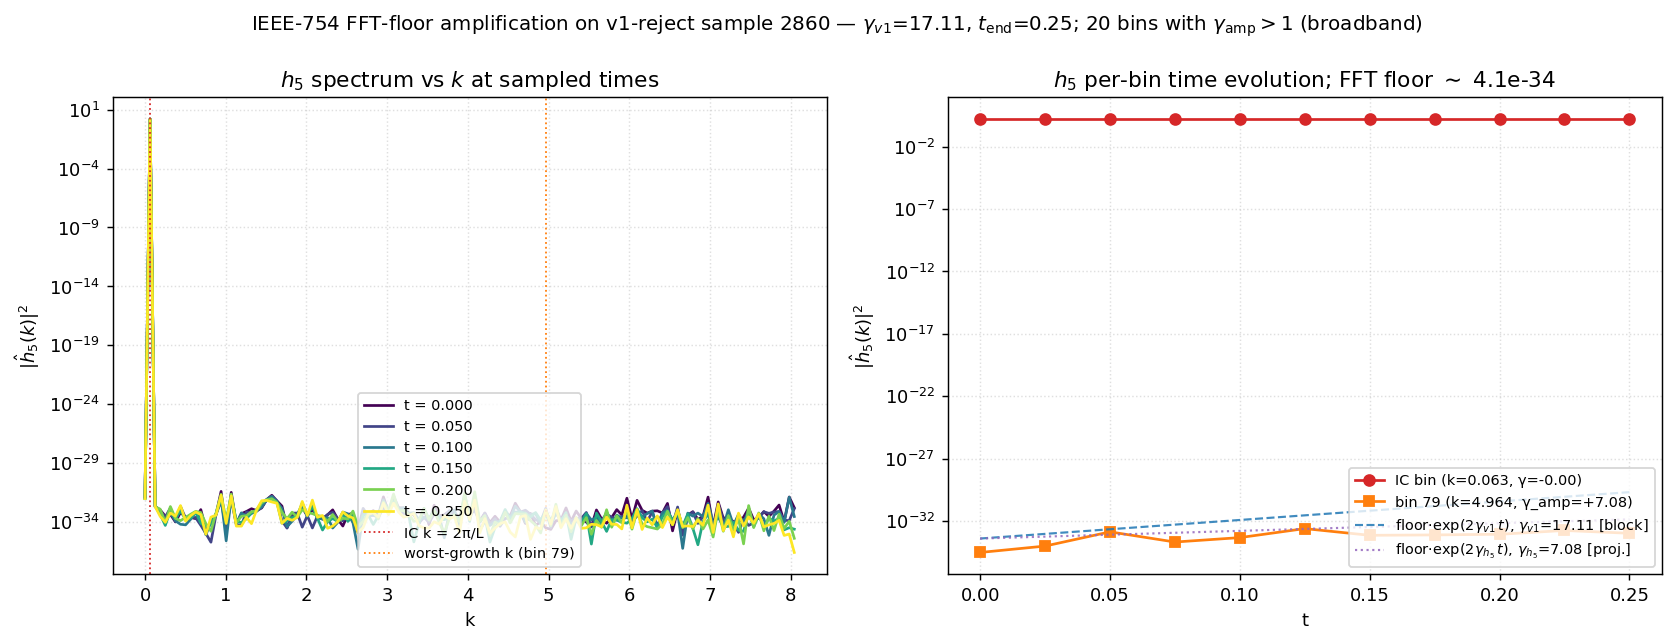
\includegraphics[width=\linewidth]{figures/probe_diagnostic_ieee_floor.png}
\caption{\textbf{Left:} per-snapshot $|\hat h_5(k)|^2$ across all
Fourier bins. The IC bin at $k = 2\pi/L \approx 0.063$ (bin~1) sits
at the expected amplitude $\sim 10^1$; every other bin sits at the
IEEE 754 FFT floor $\sim 4\times 10^{-34} \approx (10^{-2}\cdot
\varepsilon)^2$, consistent with double-precision round-off scaled
by the IC amplitude. \textbf{Right:} per-bin time evolution. The IC
bin (red) is flat ($\gamma_\mathrm{amp} \approx 0$) while the worst
non-IC bin (orange) grows at $\gamma_\mathrm{amp,\,h_5} = 7.08$.
Twenty out of $127$ non-IC bins exhibit $\gamma_\mathrm{amp} > 1$,
demonstrating broadband amplification rather than a single-bin
artefact. The blue dashed reference line $\sim
\mathrm{floor}\cdot\exp(2\gamma_{v1}\,t)$ traces the block 2-norm
growth (matching the probe's $\gamma_{v1} = 17.11$); the purple
dotted line $\sim \mathrm{floor}\cdot\exp(2\gamma_{h_5}\,t)$ traces
the source-only projection rate that h_5 actually displays.}
\label{fig:probe-diagnostic-ieee-floor}
\end{figure}

\paragraph{Source-projection effect.} Sample~2860 exhibits
$\gamma_{\mathrm{block}} = 17.11$ on the block 2-norm but
$\gamma_{\mathrm{source},\,h_5} = 7.08$ on the source-only
projection. This is not a contradiction but the expected
eigenvector-projection effect, fully analysed in
\S\ref{sec:block-norm-not-source}: the probe and the simulation's
pre-flight divergence guard both gate on the block norm, which is
why they agree, and why a hypothetical ``watch $h_5$ only''
diagnostic would under-estimate the threat. The numerical match
between the figure's blue dashed reference $\sim
\mathrm{floor}\cdot\exp(2\gamma_{v1}\,t)$ and the empirical block-
norm growth confirms the architectural invariant in practice.

\paragraph{Outcome.} The diagnostic confirms outcome (a):
\emph{IEEE-floor mechanism active}. The non-fundamental bins start
at the FFT floor and amplify exponentially; the IC bin does not
grow; the growth is broadband; the block-norm rate matches $\gamma_{v1}$.
The all-$k$ probe is mechanism-correct, not just empirically lucky.

\subsection{The $t_{\text{test}}$ choice}

The v1 probe used $t_{\text{test}} = 10$, matching the simulation's
$t_{\text{end}}$. We raise the default to $t_{\text{test}} = 20$ to
catch additional slow-growth Hwang--Noh cases inline at probe time.
The probe cost is dominated by the spectral-radius prefilter; the
longer $t_{\text{test}}$ adds at most one extra Pad\'e squaring on
the modes that survive the prefilter, an empirically measured ${\sim}5\%$
overall cost.

A residual remains: the truth-table sample 391 has
$\gamma_{\text{eff}}(t = 20) = 0.272 < 0.3$, just below the threshold.
This sample is not caught by the probe at any reasonable
$t_{\text{test}}$ within the linear-eigenvalue limit; it is caught
instead by the inline $P_{\max}$ gate after the simulation runs. The
test \texttt{tests/test\_stability.py::TestStageCTruthTable::%
test\_contamination\_caught} pins this residual via the
\texttt{KNOWN\_PROBE\_RESIDUAL} set.

\subsection{The Hwang--Noh perturbativity gate}

The Hwang--Noh perturbativity bound applies to the \emph{absolute}
conversion probability $P_{\max}$ itself: a linearised simulation
that produces $P_{\max} > 0.5$ has crossed the perturbative validity
boundary (Hwang \& Noh 2002, PRD 65, 124010), the linearised
dynamics no longer describe the underlying physics, and the value is
unreliable. This is independent of the physics quantity the user is
fitting in the likelihood. The campaign's chains typically maximise
the \emph{amplification ratio}
\begin{equation}
A = \frac{P_{\max}}{P_{\mathrm{GR}}}, \qquad
P_{\mathrm{GR}} = \sin^2\!\left(\frac{\kappa B_0\, t_{\text{end}}}{2}\right),
\end{equation}
via \texttt{--baseline-formula
"sin(kappa*B0*t\_end/2)**2"}, in which case
\texttt{compute\_log\_likelihood} returns
$\log A = \log(P_{\max} / P_{\mathrm{GR}})$. The gate condition is
nevertheless on the raw $P_{\max}$, because the perturbativity boundary
is on the absolute conversion probability, not on its ratio to
baseline; the same value of $A$ can be physical or unphysical
depending on whether $P_{\max}$ itself sits inside the linear regime.

The likelihood applies an inline gate (defined as
\texttt{P\_MAX\_LIMIT = 0.5} and the helper
\texttt{\_is\_non\_perturbative} in
\texttt{tidal/inference/\_likelihood.py}) that returns
$\log L = -\infty$ with \texttt{run\_status="non\_perturbative"} for
any sample whose raw $P_{\max}$ exceeds the limit.

The gate is applied only when the configured likelihood is
\texttt{P\_max:maximize} or \texttt{P\_max:minimize} — Gaussian-on-X
and threshold likelihoods may legitimately probe parameter regions
where $P_{\max} > 0.5$ (e.g.\ fitting a measured $P_{\max} \approx
0.6$). For maximise/minimise the metric is taken at face value (or
log-ratio'd against the baseline), so super-perturbative samples must
be rejected before they pollute the live-points pool. The cost is
one floating-point comparison per already-completed simulation.

\subsection{Inline rejection cascade}

The combined effect of probe + sim + gate is that contaminated
samples never enter the chain output. The chain CSV's
\texttt{run\_status} column carries one of
\texttt{success}, \texttt{tachyonic}, \texttt{simulation\_failed},
\texttt{metric\_missing}, \texttt{non\_perturbative}, allowing
downstream tools to distinguish each rejection mode. The
\texttt{stability\_profile} column carries the probe's stable
identifier
(\texttt{tidal.measurement.\_stability.PROBE\_PROFILE\_NAME},
currently \texttt{"unit-ic-all-k-0.3"}); bumping the probe is a
public-API change.

The post-hoc $t$-independence audit
(\texttt{tidal analyze --posthoc-audit}) remains available as a debug
tool for chains that pre-date this architecture, and as a
$2 \cdot t_{\text{base}}$ re-simulation cross-check for borderline
samples.

\subsection{References}

\begin{itemize}
\item Higham, N.J. (2009). The scaling and squaring method for the
matrix exponential revisited. SIAM Review 51(4), 747--764.
\item Higham, N.J. (2008). Functions of Matrices, SIAM, \S 2.3.
\item Hwang, J. \& Noh, H. (2002). PRD 65, 124010 — perturbativity
boundary.
\item Issue \#322: Pad\'e refactor (replaces eigenvalue+pinv approach).
\item Issue \#323: Stage C investigation (canonical probe selection).
\item \texttt{stage\_c\_truth\_table.csv} (repo root): committed
regression dataset.
\item \texttt{hpc\_results/28520217/samples.profile\_replay.csv}:
historical investigation artefact.
\end{itemize}
